% This is samplepaper.tex, a sample chapter demonstrating the
% LLNCS macro package for Springer Computer Science proceedings;
% Version 2.20 of 2017/10/04
%
\documentclass[runningheads]{llncs}
%
\usepackage{graphicx}
\usepackage{placeins}
% \usepackage{caption}
% \usepackage{subcaption}
\usepackage{amsmath}
\usepackage{hyperref}
\usepackage{xcolor}
\usepackage[linesnumbered,ruled,vlined]{algorithm2e}
\usepackage[acronym]{glossaries}

\newacronym[]{ir}{IR}{Infra Red}
\newacronym[]{fov}{FOV}{Field of View}
\newacronym[]{pdf}{PDF}{Probability Density Function}
\newacronym[]{irr}{IRR}{Infinite Impulse Response}
\newacronym[]{dof}{DOF}{Degree of Freedom}
\newacronym[]{pid}{PID}{Proportional–Integral–Derivative controller}
\newacronym[]{neat}{NEAT}{NeuroEvolution of Augmenting Topologies}

% Used for displaying a sample figure. If possible, figure files should
% be included in EPS format.
%
% If you use the hyperref package, please uncomment the following line
% to display URLs in BLUE roman font according to Springer's eBook style:
% \renewcommand\UrlFont{\color{blue}\rmfamily}
\renewcommand\UrlFont{\color{blue}\rmfamily}

\begin{document}
%
\title{Movement control of a robot through an unknown closed circuit
%\thanks{Supported by organization x.}
}
%
%\titlerunning{Abbreviated paper title}
% If the paper title is too long for the running head, you can set
% an abbreviated paper title here
%
\author{João Santos, 76912\inst{1}\orcidID{0000-0003-0393-6456
}}
%
\authorrunning{J. Santos}
% First names are abbreviated in the running head.
% If there are more than two authors, 'et al.' is used.
%
\institute{Department of Electronics, Telecommunications and Informatics \\ University of Aveiro, Portugal}
%
\maketitle              % typeset the header of the contribution
%
\begin{abstract}
In the present assignment, the challenge was to develop a robotic agent capable of going around a unknown track/maze, as fast as possible and without colliding with the walls. The agent must, also, not go backwards as that provides very few points. The best implementation was through the use of a \gls{pid} where a set of parameters were found using a genetic algorithm.

\keywords{robot, navigation, genetic algorithm, simulation, path}
\end{abstract}
%
\section{Introduction}
\label{sec:introduction}

The ability to navigate in a given environment is critical for any mobile device. The robot must first avoid risky scenarios such as collisions and unsafe conditions, but if it has a mission that requires it to visit particular locations in the robot environment, it must do so.

In the proposed assignment, a robotic agent was developed that could, autonomously and as fast as possible, go around a given map. This maps have one and only one closed loop for the robot to travel within. It must avoid collisions with the walls as that deducts points from the overall score while, also, travel in the defined forward direction (going backwards is possible, but points are awarded not every cell traveled but just every completed lap).









\section{Implementation}
\label{sec:implementation}

The developed control system resorts on a \gls{pid} to control the steering of the robot. A \gls{pid} is a feedback-based control loop mechanism which calculates an error value as the difference between a desired set-point and a measured process variable, on a continuous basis. The \gls{pid} then outputs a manipulated variable $MV$ relying on proportional, integral, and derivative terms (denoted P, I, and D, respectively), thus the name.

In general terms, the \gls{pid} control system is given by 
%
\begin{equation}
    u(t) = K_P e(t) + K_I \int_0^t e(\tau) d\tau + K_D \frac{de(t)}{dt}
\end{equation}
%
where $e(t)$ is the error and $K_P$, $K_I$ and $K_D$ are, respectively, the gains for the proportional, integral and derivative components.

With these three gains, the \gls{pid} can control the output variable with the past, present and future values of the error, like so:

\begin{itemize}
    \item Proportional: Acts upon the current value of the error. The greater the error, the greater the controller output.
    \item Integral: Takes into account previous values of the error. If there is a residual error after the proportional component, the integral term attempts to eradicate it by introducing a control effect based on the historic cumulative value of the error. 
    \item Proportional: Is the best estimate for the future direction of the error. By exerting a control influence generated by the rate of error change, it is essentially attempting to reduce the effect of the error. The faster the change, the greater the control or damping effect.
\end{itemize}

This lead us to the necessity of formulating the variable to be measured and what value we want it be have.

Given that the author can freely place the four \gls{ir} distance senors at any angle, the selected methodology consists on choosing two values, $\alpha$ and $\beta$, between 0 and 180 degrees and then placing the sensors in symmetric pairs, i.e., at $[\alpha, \beta, -\alpha, -\beta]$ degrees. This decision was taken so that an over-fit to the default map would not occur (or at least, not as easily).

With this, and assuming that the desired path for the agent is the one that leads it to be equidistant of the surrounding walls, the process variable can be computes as in equation \ref{eq:pv_formula}, where $w_i$ and $m_i$ are, respectively, the weight given to and the measure of the \gls{ir} sensor positioned at $i$ degrees. When this assumption happens to be true, in a scenario without noise in the measurements, the value of each sensor on each pair would cancel each other out, and so this formulation leads to a set-point $SP = 0$.

\begin{equation}
    PV = \sum_{i \in [\alpha, \beta, -\alpha, -\beta]} w_i \cdot m_i
    % PV = w \times \Delta \alpha + (1 - w) \times \Delta \beta
    \label{eq:pv_formula}
\end{equation}
% 
%where $\Delta \alpha$ and $\Delta \beta$ are the difference of the measures of each pair of sensors and $w \in [0, 1]$ shifts the weight towards one of the pairs.

Notice that, to maintain the desired symmetry, $w_i = -w_{-i}, i \in [\alpha, \beta]$.

\subsection{Motion Model}
\label{subsec:motion_model}

The general speed of the robot can be decomposed in the linear ($lin$) and rotational ($rot$) components, which are given by
%
\begin{equation}
    lin = \frac{out_R + out_L}{2}
\end{equation}
%
and
%
\begin{equation}
    rot = \frac{out_R - out_L}{D}
\end{equation}
%
where $out_R$ and $out_L$ are, respectively, the output speeds for the right and left wheels and $D$ is the diameter of the robot, which is unitary.

Notice that, since we define the output of the \gls{pid} as the steering control (i.e. $rot=MV$), a positive value in the output means that $out_R > out_L$ (left turn). In the same way, a negative value in the \gls{pid} output means a right turn.

All of this leads to the linear system of equation \ref{eq:linar_out_rl_basic}, that makes it possible to compute the output velocities for both wheels with only the output of the \gls{pid} and by fixing a base linear speed.

\begin{equation}
    \begin{bmatrix}
        2 lin \\
        MV
    \end{bmatrix}
    %
    =
    %
    \begin{bmatrix}
        1 & 1 \\
        1 & -1 
    \end{bmatrix}
    %
    \begin{bmatrix}
        out_R \\
        out_L
    \end{bmatrix}
    \label{eq:linar_out_rl_basic}
\end{equation}

Again, in an ideal scenario with no noise, the output of the \gls{pid} should be null on straights and different of zero on corners. To try to take advantage of this, and try to slowdown the robot on the corners and speed it up on the straights, a deduction factor (equation \ref{eq:deduction_factor}) was added to the linear system. This deduction factor is based on the last $N$ outputs of the \gls{pid} (i.e. last $N$ rotations) and also has an associated weight so its influence in the overall velocity can be fine tuned.

\begin{equation}
    d = w_d {\frac {1}{N}}\sum _{i=-1}^{-N}MV_{i}
    \label{eq:deduction_factor}
\end{equation}

Adding it all together, equation \ref{eq:linar_out_rl} outputs the desired values for each wheel.

\begin{equation}
    \begin{bmatrix}
        out_R \\
        out_L
    \end{bmatrix}
    %
    =
    %
    \begin{bmatrix}
        \frac{1}{2} & \frac{1}{2} \\
        \frac{1}{2} & -\frac{1}{2}
    \end{bmatrix}
    %
    \begin{bmatrix}
        2 lin \\
        MV
    \end{bmatrix}
    %
    +
    %
    \begin{bmatrix}
        d \\
        d
    \end{bmatrix}
    \label{eq:linar_out_rl}
\end{equation}


\subsection{Parameter Tuning}
\label{subsec_parameter_tuning}

% base_speed, P, I, D, alpha0, alpha1, w0, w1, ksr, mem_size
The formulation presented up to this point lets us with ten unknown parameters [$lin$ $K_P$ $K_I$ $K_D$ $\alpha$ $\beta$ $w_\alpha$ $w_\beta$ $w_d$ $N$]. 

The chosen method to obtain the optimal set of parameters was through the implementation of a genetic algorithm.

A genetic algorithm is a method based on natural selection, the mechanism that drives biological evolution, for addressing both constrained and unconstrained optimization problems. A population of individual solutions is repeatedly modified by the genetic algorithm. At each generation, the algorithm selects parents at random from the current population and uses them to produce the children in the next generation. The population evolves toward an optimal solution over the generations.

At each generation, the genetic algorithm has three main steps:

\begin{enumerate}
    \item Selection: performs the selection of individuals (called parents) based on their fitness score, that will contribute to the next generation.
    \item Crossover: performs the combination between two parents to form the children of the next generation.
    \item Mutation: applies random mutations to the children.
\end{enumerate}

As already mentioned, each individual must have a fitness score. This score is a value that will be used to compare it to all the others. The higher the fitness, the better. 

Typically, an individual with higher fitness has a greater change to be select as a parent than an individual with lower fitness. Notice that this does not prevent an individual with a low fitness to be selected. This is useful to maintain a diversified gene pool that together with the random mutation can, in the long run, generate a better individual.

In the proposed implementation, the fitness is the score (provided by the simulator and following the rules in it) that each individual can obtain in a fixed amount of time.

The PyGAD \cite{gad2021pygad} library was used as a basis for the genetic algorithm. It offers a base form that can be customized to fit any given optimization problem. Table \ref{tab:genetic_params} demonstrates the parameters used while table \ref{tab:gene_space} specifies the range and type for each gene. 

\begin{table}
\centering
\caption{Genetic parameter used in the evolutionary algorithm.}
\label{tab:genetic_params}
\begin{tabular}{cc}
Number generations       & 500                           \\ \hline
Solutions per population & 100                            \\ \hline
Number parents mating    & 25                             \\ \hline
Number of parents to keep    & 25                             \\ \hline
Number of genes          & 10                              \\ \hline
Parent selection type    & Steady-state selection \\ \hline
Crossover type           & Uniform                        \\ \hline
Mutation type            & Random                         \\ \hline
\end{tabular}
\end{table}

\begin{table}
\centering
\caption{Gene space for any given individual.}
\label{tab:gene_space}
\begin{tabular}{cccc}
        & Low   & High  & Data Type    \\ \cline{2-4} 
$lin$   & 0     & 1     & float   \\ \hline
$K_P$   & $- \infty$ & $+ \infty$ & float   \\ \hline
$K_I$   & $- \infty$ & $+ \infty$ & float   \\ \hline
$K_D$   & $- \infty$ & $+ \infty$ & float   \\ \hline
$\alpha$ & 0     & 180   & integer \\ \hline
$\beta$  & 0     & 180   & integer \\ \hline
$w_\alpha$     & $- \infty$ & $+ \infty$ & float   \\ \hline
$w_\beta$     & $- \infty$ & $+ \infty$ & float   \\ \hline
$w_d$     & $- \infty$ & $+ \infty$ & float   \\ \hline
$N$     & 1     & 3     & int   \\ \hline
\end{tabular}
\end{table}

\subsection{Alternative Approaches}

Additionally to the implementation described earlier, a couple of different ways were tested, yet they provided comparably worse results, maybe due too the inexperience of the author with both.

The first that we will discuss is the use of neural networks. The PyGAD library also provides a module that allows for a generic network to be "trained" using the genetic algorithm. In the attempted implementation, each chromosome was composed by two parts: i) the "optimal" angles for the \gls{ir} sensors and ii) the weights of each neuron in the network. The network would have four neurons in the input layer (one for each \gls{ir} sensor measured value) and two neurons on the output layer (the speed of each wheel). Multiple architectures were tested (no hidden layers, a single hidden layer with three or four neurons, two hidden layers with (5,3), (4,2), (3,3) neurons on each). All resulted in worse scores than the \gls{pid} implementation.

The second alternative attempt consisted on the usage of the \gls{neat} algorithm \cite{stanley:ec02}. In essence, the goal of this algorithm is to provide a "genetically evolved" neural network capable of solving a given problem. Yet, \gls{neat} not only optimizes the weight and bias of each neuron but can, also, add/remove neurons and/or connections between them. In particular, the used library, neat-python \cite{neat_python}, even allows for the activation function (among other properties) to also evolve along the generations.

\subsection{Known Issues}

Two main possible issues were detected on the developed agent.

On some corners, specially the hairpins, the robot tends to pass very close of the inner wall. Despite the fact that no collision was seen, and it is a faster path, it certainly comes with some dangers.

Similar to this on some of the ninety degree corners, as overshot may occur that lead the robot towards the outside wall. As previously, the robot is usually able to slowdown and correct the trajectory, but is also a possible collision situation.

\section{Results}
\label{sec:results}

During the run of the genetic algorithm, each individual in the population was evaluated by letting it try to obtain the highest score possible around the C1 lab provided by the described \textit{ciberRatoTools} environment. The simulation, for each individual, was over when either one thousand steps of the simulation would be completed or a wall was hit. This fitness function provided a pressure for the agents to be as fast as possible without colliding, which was the main goal of the present assignment. To build a more robust agent, the training environment had higher noise levels then the evaluation one. This option was taken after the evolved agents with the standard noise values, in certain circumstances, would hit the wall. This behaviour drastically decreased after the agents were tested in a noisier environment.

Figure \ref{fig:evolution_by_generation} shows the evolution of the score along the generations. It very clearly shows that, by pure chance, very early a big leap in fitness score was achieved that took the best solution too obtain a score of almost six hundred points (i.e. the robot traveled almost sixty cells within the stipulated time). Over time, the fitness floated, but tended towards a stagnation around the 680 value.

\begin{figure}
    \centering
    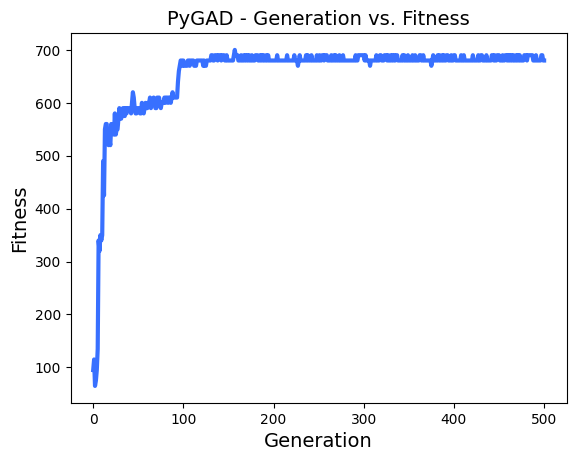
\includegraphics[width=\textwidth]{imgs/graph_690_2022.01.27_16.53.06.png}
    \caption{Evolution of the fitness value of the best individual in each generation.} 
    \label{fig:evolution_by_generation}
\end{figure}
\FloatBarrier

After all the generations, the best solutions was
%
\begin{equation*}
    \begin{bmatrix}
        lin \\
        K_P \\
        K_I \\
        K_D \\
        \alpha \\
        \beta \\
        w_\alpha \\
        w_\beta \\
        w_d \\
        N
    \end{bmatrix}
    %
    =
    %
    \begin{bmatrix}
        0.189068 \\
        7.740097 \\
        0.681015 \\
        -0.007488 \\
        36 \\
        42 \\
        0.851787 \\
        0.758472 \\
        0.480972 \\
        1
    \end{bmatrix}
\end{equation*}
%
and the ability to reach a score of 3540 when allowed to run for the full five thousand simulator steps.

Two particularities caught the attention of the author:
%
\begin{enumerate}
    \item although the initial idea was for $w_\alpha$ and $w_\beta$ to provide a weighted average, the fact is that, on the best solution, $w_\alpha+w_\beta>1$;
    \item the best solution "opted" to use as little knowledge about the past as possible ($N=1$), but it was still useful since it gave it a non-zero weight $w_d$.
\end{enumerate}




Finally, a couple of videos are provided of the developed agent running on the C1 lab and on another one developed by the author:
%
\begin{itemize}
    \item \url{https://youtu.be/jJx0Y6EDXHQ}
    \item \url{https://youtu.be/Wgdqme6gSD8}
\end{itemize}


\section{Conclusion}

The developed agent is, has intended, able to move around the map without colliding with the walls and so, the major goal of this assignment has been accomplished. The author acknowledges that faster ways could exist, but given the tries he made, the \gls{pid} ended up being the most reliable one.



%
% ---- Bibliography ----
%
% BibTeX users should specify bibliography style 'splncs04'.
% References will then be sorted and formatted in the correct style.
%
\bibliographystyle{splncs04}
\bibliography{bib}
%
\end{document}
